\documentclass{standalone}
\usepackage{tikz}
\usepackage{ctex,siunitx}
\usepackage{tkz-euclide}
\usepackage{amsmath}
\usetikzlibrary{patterns, calc}
\usetikzlibrary {decorations.pathmorphing, decorations.pathreplacing, decorations.shapes,}
\begin{document}
\small
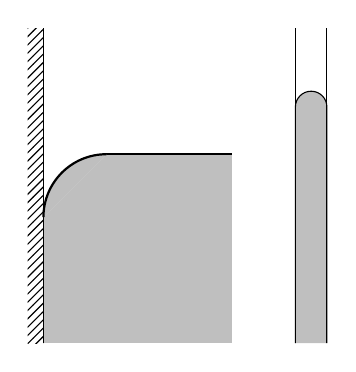
\begin{tikzpicture}[>=stealth,scale=0.8]
  \fill [gray!50] (0,0) rectangle (3,2);
  \fill [gray!50] (1,2) rectangle (3,3);
  \fill [gray!50] (0,2)--(1,3)--(1,2);
  \draw[ thick ](1,3)--(3,3);
  \draw [fill=gray!50, thick ](1,3) arc(90:180:1);
  \fill [white] (4, 0) rectangle (4.5, 5);
  \draw [fill=gray!50, rounded corners=0.2cm](4.5, 0)--(4.5, 4)--(4,4)--(4,0);
  \draw (4, 0)--(4,5);
  \draw (4.5, 0)--(4.5,5);
  \fill [pattern=north east lines](-.25,0) rectangle(0,5);
  \draw (0,0)--(0,5);
\end{tikzpicture}
\end{document}